\section{Bootstrap support (BS) values of the central branch $AB$ of the $16$-taxon tree as in Fig.\,\ref{fig:simulation}b for $n =100$ number of sites.}

%%% Tab. Bootstrap values %%%
\begin{table}[hb]
    \centering
    \begin{tabular}{|c|c|c|c|c|}
\hline
Branch & $AB$ split & Average  & Minimum & \% Informative\\
Length & contained   & BS value & BS value & instances \\
\hline
0.1 &  993 &  93.32 &  14 & 100   \\
0.2 &  999 &  99.19 &  74 & 100   \\
0.3 & 1000 &  99.86 &  87 & 100   \\
0.4 & 1000 &  99.95 &  93 & 100   \\
0.5 & 1000 &  99.99 &  97 & 100   \\
0.8 & 1000 & 100    & 100 &  99.1 \\
1   & 1000 & 100    & 100 &  92.4 \\
1.5 & 1000 & 100    & 100 &  49.7 \\
2   & 1000 & 100    & 100 &  21.6 \\
2.5 & 1000 & 100    & 100 &   9.6 \\
3   & 1000 & 100    & 100 &   5.9 \\
3.5 & 1000 & 100    & 100 &   4.3 \\
4   & 1000 & 100    & 100 &   4.6 \\
5   & 1000 & 100    & 100 &   3.8 \\
7.5 & 1000 & 100    & 100 &   3.5 \\
10  & 1000 & 100    & 100 &   4.3 \\
\hline
    \end{tabular}
    \vspace{0.25cm}
    \caption{
\textbf{Bootstrap support (BS) values of the central branch $AB$ of the $16$-taxon tree as in Fig.\,\ref{fig:simulation}b for $n =100$ number of sites.} For each Branch length of $AB$, $1000$ alignments were simulated and used to ML-estimate $1000$ trees. Only ML-trees with a branch splitting the taxa of $\mathbb{T}_A$ and $\mathbb{T}_B$ were considered ($AB$ split contained). For each considered tree, the BS value of this splitting branch using $100$ resamplings was computed, allowing to compute the Average BS value and Minimum BS value using all considered trees. For comparison, we include the percentage of Informative instances of Fig. \ref{fig:simulation}.b for $n=100$ and Bonferroni-corrected ML-tree (dashed line, {\color{britishracinggreen} dark green}). The case $n=1000$ and $n=10000$ sites is not represented because all branch lengths had $1000$ trees containing the $AB$ split and a minimum BS value of $100$.
    }
    \label{tab:bootstrap}
    \end{table}

    \clearpage

%%% currently Fig S1. (model mis-specification) %%%
\begin{figure}[H]
        \centering
        
\includegraphics[width=\linewidth]{figure_simulated_data_misspecification.pdf}
        		     \caption{\textbf{Performance of Satute in presence of model mis-specification.} Fraction of informative instances (i.e. $H_0$ rejected) plotted as a function of the length of the tested branch $AB$ in either the true tree ({\color{red}light red}), the true topology with ML branch lengths ({\color{burgundy} dark red}), the ML tree ({\color{applegreen} light green}) or the ML tree with Bonferroni-corrected test ({\color{britishracinggreen} dark green}).
       The branches tested were \textbf{(a-c)} the external branch $AB$ of a $5$-taxon tree and \textbf{(d-f)} the central branch $AB$ of a balanced $16$-taxon tree. Dashed, solid and alternating dashed lines represent the results for alignments with $100, 1000$ and $10000$ number of sites, respectively. 
       In all cases the alignments were simulated with a GTR model, while reconstruction and testing was performed using the JC \textbf{(a,d)}, K2P \textbf{(b,e)} or F81 \textbf{(c,f)}. 
       For further details see the Protocol sections.}
	\label{fig:simulation_misspec}
 \end{figure}

%%%%% Fig S1a-c - model misspecification simulation A4-B1 %%%%%
\subsection*{Protocol for Supplementary Fig.\,\ref{fig:simulation_misspec}a-c}\label{subsec:misspec_5tree}

This protocol mostly follows the protocol of Fig.\,\ref{fig:simulation}a.

\medskip

\noindent In the 5-taxon tree (shown in Fig.\,\ref{fig:simulation}a), one taxon $B$ was connected to the root $A$ of a balanced 4-taxon subtree $\mathbb{T}_A$. All branch lengths in $\mathbb{T}_A$ equalled 0.2, while the branch lengths of $AB$ varied from $\{0.1, 0.2, 0.3, 0.4, 0.5, 0.8, 1.0, 1.5, 2.0, 2.5, 3.0, 3.5, 4.0, 5.0, 7.5, 10.0\}$. For each parameterisation we simulated sets of $1000$ DNA alignments with ${n = 100, 1000, 10000}$ sites using Seq-Gen \citep[v1.3.4;][]{Rambaut1997}
using a GTR model with rates $AC=0.6676$, $AG=3.7807$, $AT=4.2833$, $CG=0.5354$, $CT=0.8718$ and $GT=1.0$ and nucleotide frequencies $\pi_A = 0.125$, $\pi_C = 0.436$, $\pi_G = 0.191$ and $\pi_T =0.245$, as estimated for the best-fit model for the dataset PF06346 stored in the EvoNAPS database.
Alignments were evaluated using IQ-Tree 2.2.2.7 and Satute with significance level $\alpha = 0.05$ while specifying JC \textbf{(a)}, K2P \textbf{(b)} and F81 \textbf{(c)} as models of substitution instead of GTR. Missing model parameters are estimated from the alignments.

\medskip
The fraction of informative instances (rejection of $H_0$) is plotted as a function of the branch length $AB$ for four analyses:

\medskip

\begin{itemize}
  \item Using the true simulation tree with fixed true branch lengths ({\color{red}light red}).
  \item Using the true tree topology with ML-estimated branch lengths ({\color{burgundy} dark red}).
  \item Using the ML-estimated tree and estimated branch lengths ({\color{applegreen} light green}).
  \item Using the ML-estimated tree with estimated branch lengths plus Bonferroni correction $\alpha_{COR} = \alpha/4$ ({\color{britishracinggreen} dark green}).
\end{itemize}

\medskip

Since the JC \textbf{(a)} and the F81 \textbf{(c)} models have a unique non-zero eigenvalue with multiplicity $3$, we used statistic $\hat{\delta} = \hat{C}_1+\hat{C}_2+\hat{C_3}$ (Supplementary Eq. \ref{eq:dominant_coherence}). Node $B$ is external, and thus the uncorrected tests ({\color{red}light red}, {\color{burgundy} dark red} and {\color{applegreen} light green}) reject independence if 
\begin{equation}
  \hat{\delta} > z_\alpha \frac{
    \sqrt{
      \hat{\sigma}^2_{A,1}+\hat{\sigma}^2_{A,2}+\hat{\sigma}^2_{A,3}
    }
  }{\sqrt{n}}
\end{equation}
for $\alpha=0.05$, while $\alpha_{COR}=0.05/4$ (Supplementary Eq. \ref{eq:threshold_D_external}) is used for the corrected test ({\color{britishracinggreen} dark green}). The largest nonzero eigenvalue under the K2P model \textbf{(b)} has multiplicity $2$, and thus we used statistic $\hat{\delta} = \hat{C}_1+\hat{C}_2$ (Supplementary Eq. \ref{eq:dominant_coherence}), giving for the uncorrected tests ({\color{red}light red}, {\color{burgundy} dark red} and {\color{applegreen} light green}) a rejection of independence if 
\begin{equation}
  \hat{\delta} > z_\alpha \frac{
    \sqrt{
      \hat{\sigma}^2_{A,1}+\hat{\sigma}^2_{A,2}
    }
  }{\sqrt{n}}
\end{equation}
for $\alpha=0.05$, while $\alpha_{COR}=0.05/4$ (Supplementary Eq. \ref{eq:threshold_D_external}) is used for the corrected test ({\color{britishracinggreen} dark green}).


%%%%% Fig S1d-f - model misspecification simulation A8-B8 %%%%%
\subsection*{Protocol for Supplementary Fig.\,\ref{fig:simulation_misspec}d-f}\label{subsec:misspec_16tree}
This protocol mostly follows the protocol of Fig.\,\ref{fig:simulation}b.

\medskip

In the 16-taxon tree (shown in Fig.\,\ref{fig:simulation}b), the root $A$ of a balanced $8$-taxon subtree $\mathbb{T}_A$ was connected to the root $B$ of a balanced $8$-taxon subtree $\mathbb{T}_B$. The branch lengths for the internal and external branches of subtrees $\mathbb{T}_A$ and $\mathbb{T_B}$ were drawn from the distributions of all internal and external branch lengths, respectively, as stored in the EvoNAPS database (Reden, 2023; http://evonaps.cibiv.univie.ac.at) for the sources OrthoMaM, Lanfear and TreeBase. Branch lengths were sampled between $0.04$ and $0.2$. Branch lengths $AB$ equaled $\{0.1, 0.2, 0.3, 0.4, 0.5, 0.8, 1.0, 1.5, 2.0, 2.5, 3.0, 3.5, 4.0, 5.0, 7.5, 10.0\}$. 
For each parameterisation we simulated sets of $1000$ DNA alignments with $n = 100, 1000, 10000$ sites using Seq-Gen \citep[v1.3.4;][]{Rambaut1997} 
using a GTR model with rates $AC=0.6676$, $AG=3.7807$, $AT=4.2833$, $CG=0.5354$, $CT=0.8718$ and $GT=1.0$ and nucleotide frequencies $\pi_A = 0.125$, $\pi_C = 0.436$, $\pi_G = 0.191$ and $\pi_T =0.245$ as estimated for the best-fit model for the dataset PF06346 as stored in the EvoNAPS database.
Alignments were evaluated using IQ-Tree 2.2.2.7 and Satute with significance level $\alpha = 0.05$ while specifying JC \textbf{(a)}, K2P \textbf{(b)} and F81 \textbf{(c)} as models of substitution instead of GTR. Missing model parameters are estimated from the alignments.

\medskip

Again the fraction of informative instances (rejection of $H_0$) is plotted as a function of the branch length $AB$ for four analyses:

\medskip

\begin{itemize}
  \item Using the true simulation tree with fixed true branch lengths ({\color{red}light red}).
  \item Using the true tree topology with ML-estimated branch lengths ({\color{burgundy} dark red}).
  \item Using the ML-estimated tree and estimated branch lengths ({\color{applegreen} light green}).
  \item Using the ML-estimated tree with estimated branch lengths plus Bonferroni correction $\alpha_{COR} = \alpha/64$ ({\color{britishracinggreen} dark green}).
\end{itemize}

\medskip

{\color{red}Each datapoint in Fig.\,\ref{fig:simulation}b has been computed from an independent set of $1000$ alignments. DISCARDED ALIGNMENTS.}

\medskip

Since the JC \textbf{(a)} and the F81 \textbf{(c)} models have a unique non-zero eigenvalue with multiplicity $3$, we used statistic $\hat{\delta} = \hat{C}_1+\hat{C}_2+\hat{C_3}$ (Supplementary Eq. \ref{eq:dominant_coherence}). Branch $AB$ is internal, and thus the uncorrected test ({\color{red}light red}, {\color{burgundy} dark red} and {\color{applegreen} light green}) is stated in Supplementary Eq. \ref{eq:th_zscore}, namely
\begin{equation}
     \hat{\delta} >  z_\alpha \frac{\sqrt{\sum_{k, l \in [3]} 
   \hat{K}^A_{kl}   \hat{K}^B_{kl}.
}}{\sqrt{n}},
\end{equation} 
for $\alpha=0.05$ or $\alpha_{COR}=0.05/64$ (Supplementary Eq. \ref{eq:threshold_D_external}) for {\color{britishracinggreen} dark green}. The largest nonzero eigenvalue under the K2P model \textbf{(b)} has multiplicity $2$, and thus we we used statistic $\hat{\delta} = \hat{C}_1+\hat{C}_2$ (Supplementary Eq. \ref{eq:dominant_coherence}), giving for the uncorrected tests ({\color{red}light red}, {\color{burgundy} dark red} and {\color{applegreen} light green}) a rejection of independence if 
\begin{equation}
     \hat{\delta} >  z_\alpha \frac{\sqrt{\sum_{k, l \in [2]} 
   \hat{K}^A_{kl}   \hat{K}^B_{kl}.
}}{\sqrt{n}} = z_\alpha \frac{\sqrt{
\hat{\sigma}^2_{A,1}\hat{\sigma}^2_{B,1}+\hat{\sigma}^2_{A,2}\hat{\sigma}^2_{B,2} + 2\hat{K}^A_{12}\hat{K}^B_{12}.
}}{\sqrt{n}},
\end{equation}
for $\alpha=0.05$, while $\alpha_{COR}=0.05/64$ (Supplementary Eq. \ref{eq:threshold_D_external}) is used for the corrected test ({\color{britishracinggreen} dark green}).

\bigskip

% currently Fig S2 (A8-B8, min blen 1/seqlen)
\begin{figure}[H]
            \centering
            \includegraphics[scale=0.5]{figure_simulated_data_s2.pdf}
                       \caption{\textbf{Effect of short branches on the Bonferroni-corrected test for saturation using simulated data.}
                       The fraction of informative instances (i.e. H0 rejected) is plotted as a function of the length of the tested branch AB in either the true tree ({\color{red}light red}), the true topology with ML-lengths ({\color{burgundy} dark red}), the ML-tree ({\color{applegreen} light green}) or the ML tree with Bonferroni-corrected test ({\color{britishracinggreen} dark green}). Dashed, solid and alternating dashed lines represent the results for alignment lengths $100, 1000$ and $10000$, respectively. For large central branch lengths, the type I error rate of the Bonferroni-corrected test ({\color{britishracinggreen} dark green}) is smaller than the significance level $\alpha = 5\%$.
                       }
	\label{fig:simulation_shortBranches}
\end{figure}

\color{black}


\subsection*{Protocol for Supplementary Fig.\,\ref{fig:simulation_shortBranches}}We closely followed the Protocol for Fig.\,\ref{fig:simulation}b. The only difference was that, for the internal and external branch lengths, a lower minimum length of $1/n$ (instead of $0.04$) was used, where $n$ is the length of the alignment.

\newpage

\begin{table}[h!]
     \centering 
    \begin{tabular}{|c|c|c|c|c|c|c|c|}
      \hline
       Protein & \# Sites & \# Seqs. & \# Tested  &\multicolumn{3}{c|}{\# Saturated branches}\\
& $n$ & of gaps &branches& Internal & External & Total\\
\hline
L2  & 317 &  27 & 6110 &  0 &  55 &  55\\
L3  & 228 & 139 & 5886 &  2 &  43 &  45\\
L4  & 245 & 111 & 5942 &  0 &   0 &   0\\
L5  & 164 &  91 & 5982 &  0 &  18 &  18\\
L6  & 220 &  31 & 6102 &  1 &  65 &  66\\
L14 & 125 &  49 & 6066 &  0 &   0 &   0\\
L15 & 122 &  18 & 6128 & 14 & 136 & 150\\
L16 & 153 &  85 & 5994 & 60 & 132 & 192\\
L18 & 141 &  64 & 6036 &  6 &  50 &  56\\
L22 & 174 &  55 & 6054 &  0 &  45 &  45\\
L24 &  81 &  89 & 5986 &  0 &   3 &   3\\
S3  & 216 &  48 & 6068 & 24 & 113 & 137\\
S8  & 141 &  32 & 6100 &  2 &  98 & 100\\
S10 & 104 & 419 & 5326 &  0 &   0 &   0\\
S17 &  74 & 195 & 5775 &  2 &  23 &  25\\
S19 &  91 & 163 & 5838 & 16 & 109 & 125\\
\hline
     \end{tabular}
     \vspace{0.25cm}
     \caption{ \textbf{Per-protein summary of saturation in the tree of life represented in Fig.\,\ref{fig:tree_of_life_saturated_branches}.} For each ribosomal protein, the table includes the number of sites in the corresponding subalignment (\# Sites $n$), the number of sequences in this subalignment that are compposed uniquely by gaps (\# Seqs. of gaps), the number of branches that were tested by Satute after pruning all taxa composed uniquely by gaps (\# Tested branches),  and the number of Saturated branches for Internal branches, External branches and both (Total).}
	\label{table:per_protein_summary}
    \end{table}

\noindent \textbf{Protocol for Table \ref{table:per_protein_summary}:} See the Protocol for Fig.\,\ref{fig:tree_of_life_saturated_branches}

\newpage

     \begin{table}[h!]
    \centering
    \begin{tabular}{|c|c|c|c|}
\hline
Protein & Z-score  & Z-score & $\Delta$ Z-score \\
       & Eukaryota & yeast & (Euk.- Yeast)\\
\hline
L2  & 11.68 & 12.85 & -1.17\\
L3  & 11.62 & 11.38 &  0.24\\
L4  & 11.06 & 12.23 & -1.17\\
L5  & 12.31 & 12.54 & -0.23\\
L6  & 10.34 & 10.49 & -0.15\\
L14 &  9.96 & 10.47 & -0.51\\
L15 &  7.72 &  8.88 & -1.16\\
L16 &  6.35 & 11.30 & -4.95 \\
L18 &  8.23 & 11.82 & -3.59\\
L22 &  8.28 & 11.70 & -3.42\\
L24 &  7.77 &  7.55 &  0.22\\
S3  & 10.85 & 12.81 & -1.96\\
S8  & 10.03 & 10.48 & -0.45\\
S10 &  8.91 &  9.15 & -0.24\\
S17 &  7.92 &  7.23 &  0.69\\
S19 &  8.35 &  8.49 & -0.14\\
\hline

    \end{tabular}
    \vspace{0.25cm}
    \caption{\textbf{Per-protein Satute z-score for two branches of a given tree.} For each ribosomal protein, Satute z-score of the branch leading to Eukaryota and yeast in the 2D-tree of Fig.\,\ref{fig:EUK}a. Their differences ($\Delta$ Z-score) are represented in Supplementary Fig.\, \ref{fig:Eukaryota_Yeast}.}
    \label{tab:Eukaryota_Yeast}
    \end{table}

\begin{figure}[h!]
            \centering
            
\includegraphics[width=0.6\linewidth]{protein_based_comparison_Yeast_Eukaryota_diff_zscores.pdf}
		     \caption{\textbf{Per-protein Satute z-score difference between the branches leading to Eukaryota and yeast.} For each protein of the ribosomal protein alignment, difference in the Satute z-score between the branch leading to Eukaryotes and the branch leading to yeast in the 2D-tree of \mbox{Fig.\,\ref{fig:EUK}a.} }
		     \label{fig:Eukaryota_Yeast}
        \end{figure}

\noindent \textbf{Protocol for  Table \ref{tab:Eukaryota_Yeast}  and Fig.\,\ref{fig:Eukaryota_Yeast}}:
 To examine the variations in protein sequences between evolutionary branches leading to Eukaryota and baker's yeast (S. cerevisiae), we first identify the specific branches of interest in the ML-reconstructed 2D tree (referenced as Fig.\,\ref{fig:EUK}a). Subsequently, Satute is employed to conduct a thorough evolutionary analysis on these selected branches, utilizing the protein alignment alongside the phylogenetic tree provided. The protein evolutionary model used is LG+G4. From the output generated by Satute, we compute z-scores of the selected branches for different proteins, where the specific proteins are defined by a given annotation file. The z-score calculations follow the method outlined in the protocol for Figs. \ref{fig:EUK}c, \ref{fig:EUK}f  and the results are aggregated and presented in Table \ref{tab:Eukaryota_Yeast}. To visualize the differences in the z-scores across proteins, a customized R script is used, facilitating the interpretation of evolutionary patterns and divergence between the branches leading to Eukaryota and S. cerevisiae.

        
\noindent \textbf{Protocol for  Table \ref{tab:Eukaryota_Yeast}  and Fig.\,\ref{fig:Eukaryota_Yeast}}: For the protein-based 2D tree, Satute assigned one rate category to each site, then computed the scalar product $C_1^\partial$  and the one-site standard deviation  $\hat{\sigma}_1$ as explained in the protocol of Fig.\,\ref{fig:EUK}.c,f. For each protein, the estimate $\hat{C}_1$ was computed, giving the z-score $\sqrt{n}\hat{C}_1/\hat{\sigma}_1$, where $n$ is the number of sites in the protein considered. 

\medskip

The rearranged protein-based tree of Supplementary Fig.\,\ref{fig:rearrangedtree} was constructed manually, while its branch lengths were ML-estimated using IQ-Tree2, as also the parameters of model GTR+G4. A z-score $\sqrt{n}\hat{C}_1/\hat{\sigma}_1$ for each protein was obtained as we did for the protein-based 2D tree.

\newpage


\begin{table}[h!]
    \centering
    \begin{tabular}{|c|c|c|c|}
\hline
Protein& Z-score & Z-score& $\Delta$ Z-score\\
&2D tree & 3D-rear. & (2D-3D)\\
\hline
L2&11.68&11.65& 0.03\\
L3&11.62&11.07& 0.55\\
L4&11.06&11.02& 0.04\\
L5&12.31&12.21& 0.10\\
L6&10.34&10.27& 0.07\\
L14&9.96&9.01& 0.95\\
L15&7.72&8.75& -1.03\\
L16&6.35&6.30& 0.05\\
L18&8.23&8.11& 0.12\\
L22&8.28&8.69& -0.41\\
L24&7.77&7.68& 0.09\\
S3&10.85&10.51& 0.34\\
S8&10.03&9.77& 0.26\\
S10&8.91&9.04& -0.13\\
S17&7.92&7.37& 0.55\\
S19&8.35&8.01& 0.34\\
\hline
    \end{tabular}
    \vspace{0.25cm}
    \caption{\textbf{Per-protein Satute z-score for the branch leading to Eukaryota in two different trees.} For each ribosomal protein, Satute z-score of the branch leading to Eukaryota in the 2D-tree of Fig.\,\ref{fig:EUK}a and the 3D-rearranged tree of Fig.\,\ref{fig:z-score_differences}a. The sorted difference in z-score between the 2D and 3D-rearranged tree for the branch leading to Eukaryote ($\Delta$ Z-score) is represented in Fig.\, \ref{fig:z-score_differences}.b.}
    \label{tab:protein_2D_3D}
    \end{table}

\noindent  \textbf{Protocol for  Table \ref{tab:protein_2D_3D}}: See the Protocol for Fig.\,\ref{fig:z-score_differences}b.
\newpage 

    \begin{table}[ht]
    \centering
\begin{tabular}{ | m{3cm} | m{2cm}| }  
  \hline
  Proteins included & $L_{2D}-L_{3D}$\\ 
  \hline
  L15, L22, S10, L2 & -32.83 \\ 
  \hline
  + L4 & -7.10 \\ 
   \hline
  + L16 & 11.84 \\ 
   \hline
  + L15 & 17.12 \\ 
  \hline
\end{tabular}
\caption{Difference in log-likelihood between the 2D-tree and the rearranged 3D-tree for different subalignments. We progressively extend the original alignment of proteins L15, L22, S10, L2  by adding the next protein with the minimum difference in Satute z-score (Fig.\,\ref{fig:difference}). The topologies were fixed as described in Fig.\,\ref{fig:2DTREE} for the 2D-tree and in Fig.\,\ref{fig:rearrangedtree} for the rearranged 3D-tree, while branch lengths were ML-estimated. }
\label{table:1}
\end{table}

{\color{red}why this selection}

\clearpage

{\color{olive} \textbf{Suggestion from Christiane: START}\\
\begin{figure}[H]
\centering
            \includegraphics[width=0.8\linewidth]{rearranged_rRNA_2D_tree.pdf}
                       \caption{{\color{olive}Simplified diagram of the topology rearrangement of the rRNA-based  3D tree of Fig.\,\ref{fig:EUK}c into a 2D tree, with branch lengths ML-optimised by replacing the black dashed branch with the green dashed branch.}}
	\label{fig:rRNA_rearranged2Dtree}
\end{figure}

\noindent  \textbf{Protocol for  Table \ref{tab:rRNA_2D_3D}  and Fig.\,\ref{fig:rRNA_2D_3D}}:
To elucidate the effects of tree topology on rRNA sequence evolution, we undertake an analytical comparison between rRNA sequences positioned within both original 3D and topologically rearranged 2D ML-optimised  phylogenetic trees. Initial identification of relevant branches is carried out using an established 3D tree (depicted in Fig.\,\ref{fig:EUK}d) and a newly arranged 2D tree (illustrated in Fig.\,\ref{fig:rRNA_rearranged2Dtree}). Employing Satute, we perform a detailed evolutionary analysis for these specific branches using the corresponding rRNA alignments and phylogenetic trees. The chosen evolutionary model for this analysis is GTR+G4. Outputs from Satute are then utilized to compute z-scores for various rRNA regions, categorized according to an rRNA region annotation file. These computations adhere to methodologies specified for Figs. \ref{fig:EUK}c and \ref{fig:EUK}f, with results aggregated and displayed in Table \ref{tab:rRNA_2D_3D}. To enhance the interpretation of differences influenced by tree topology, a customized R script visualizes the z-score discrepancies between the 2D and 3D tree analyses, elucidating potential variances in protein evolutionary patterns due to tree topology.

\newpage

\begin{figure}[H]
            \centering
            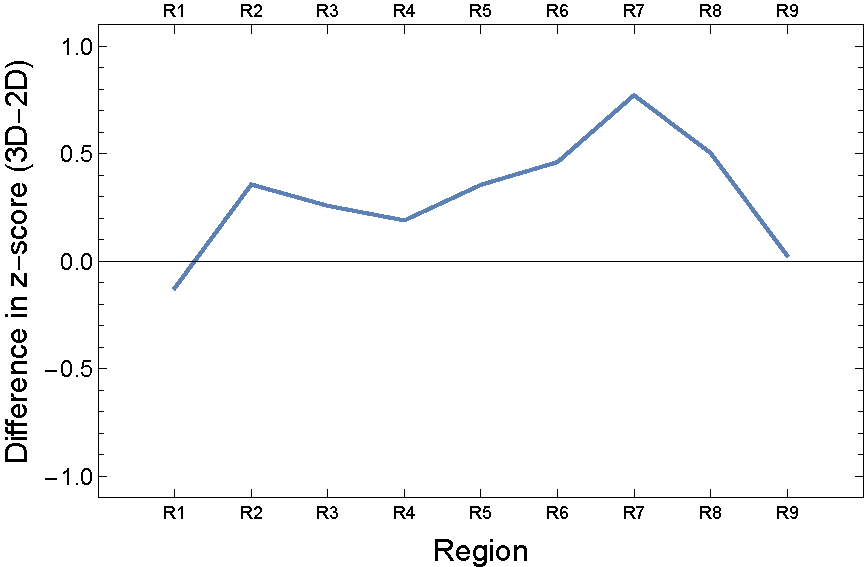
\includegraphics[width=0.8\linewidth]{zScoreByRegion.pdf}
		     \caption{{\color{red}Was the bar diagram updated after the bug? }}
		     \label{fig:difference16S}
        \end{figure}

    \begin{table}[h!]
    \centering
    \begin{tabular}{|c|c|c|}
\hline
Region & Z-score 3D tree & Z-score 2D-rearranged tree\\
\hline
R1&4.57&5.08\\
R2&6.12&5.94\\
R3&3.62&3.45\\
R4&6.80&6.83\\
R5&8.99&8.93\\
R6&8.54&8.31\\
R7&8.93&8.35\\
R8&12.44&12.32\\
R9&9.32&9.65\\
\hline
    \end{tabular}
    \vspace{0.25cm}
    \caption{{\color{olive}\textbf{Per-protein z-scores} for the branches leading to Eukaryota in the ML-reconstructed 3D tree (Fig.\,\ref{fig:EUK}c) and the rearranged 2D tree (Supplementary Fig.\,\ref{fig:rRNA_rearranged2Dtree})}}
    \label{tab:rRNA_2D_3D}
    \end{table}

\begin{figure}[H]
            \centering
            \includegraphics[width=0.8\linewidth]{rRNA_based_comparison_2D_3D_diff_zscores.pdf}
		     \caption{{\color{olive}\textbf{Per-protein z-scores comparison to a rearranged topology.} For each protein of the protein alignment, difference in the Satute z-score in the branch leading to Eukaryota between the ML-reconstructed 3D tree (Fig.\,\ref{fig:EUK}c) and the rearranged 2D tree (Supplementary Fig.\,\ref{fig:rRNA_rearranged2Dtree}). }}
		     \label{fig:rRNA_2D_3D}
        \end{figure}

\textbf{Suggestion from Christiane: END}}\\


\clearpage

\iffalse 

\begin{figure}[H]
            \includegraphics[width=0.8\linewidth]{indexFigure.pdf}
                       \caption{For the 16S rRNA gene alignment, plots of the z-scores obtained from sliding-window testing ($n=36$) using Satute in the branch leading to Eukaryotes (purple) and the branch-independent saturation index (blue). Grey shadows indicate regions where the branch leading to Eukaryotes is affected by saturation, while the saturation index rejects saturation.}
	\label{fig:indexFigureRNA}
\end{figure}

\begin{figure}[H]
            \includegraphics[width=0.8\linewidth]{indexAA.pdf}
                       \caption{For the ribosomal protein alignment, plots of the z-scores obtained from from sliding-window testing ($n=36$) using Satute in the branch leading to Eukaryotes (purple) and the branch-independent saturation index (blue).}
	\label{fig:indexFigureAA}
\end{figure}

\fi


\end{appendices}
%%==============================================================================